\section{Multi-Graph Matching}
\label{sec:multi-graph-matching}
The multi-graph matching problem is an extension of the graph matching problem from Section~\ref{sec:graph-matching} to more than two graphs with additional cycle consistency constraints ensuring that compositions of matchings are consistent.

\begin{definition}[Multi-Graph Matching]
Given $N_1,\ldots,N_K > 0$ and linear costs $c^{pk} \in \R^{N_p \times N_k}$ and quadratic costs $d^{pk} \in \R^{N_p \times N_k \times N_p \times N_k}$ for every $p < k$, the multi-graph matching problem is
\begin{equation}
\begin{array}{cl}
    \min\limits_{(x^{pk} \in \R^{N_p \times N_k})_{p,k}}
    &\sum\limits_{p < k} \sum\limits_{ij \in E} c_{ij} x_{ij} + \sum\limits_{ijkl \in T} d_{ijkl} x_{ij} x_{kl} \\ 
\text{s.t.}
& \sum\limits_{j=1,\ldots,m} x^{pk}_{ij} \leq 1 \quad \forall i\in [N_p], p < k \\
& \sum\limits_{i=1,\ldots,n} x^{pk}_{ij} \leq 1 \quad \forall j\in [N_k], p < k \\
& x^{pk} \cdot x^{kl} \leq x^{pl} \quad \forall p \neq k \neq l \\
    & x^{pk} = (x^{kp})^\top \quad \forall p \neq k
\end{array}
\end{equation}
where we use~$\cdot$~for matrix multiplication and~$\leq$~holds elementwise.
\end{definition}

An illustration of the multi-graph matching problem with matchings that obey resp.\ violate cycle consistency is given in Figure~\ref{fig:multi-graph-matching}.

\begin{figure}[H]
    \centering
    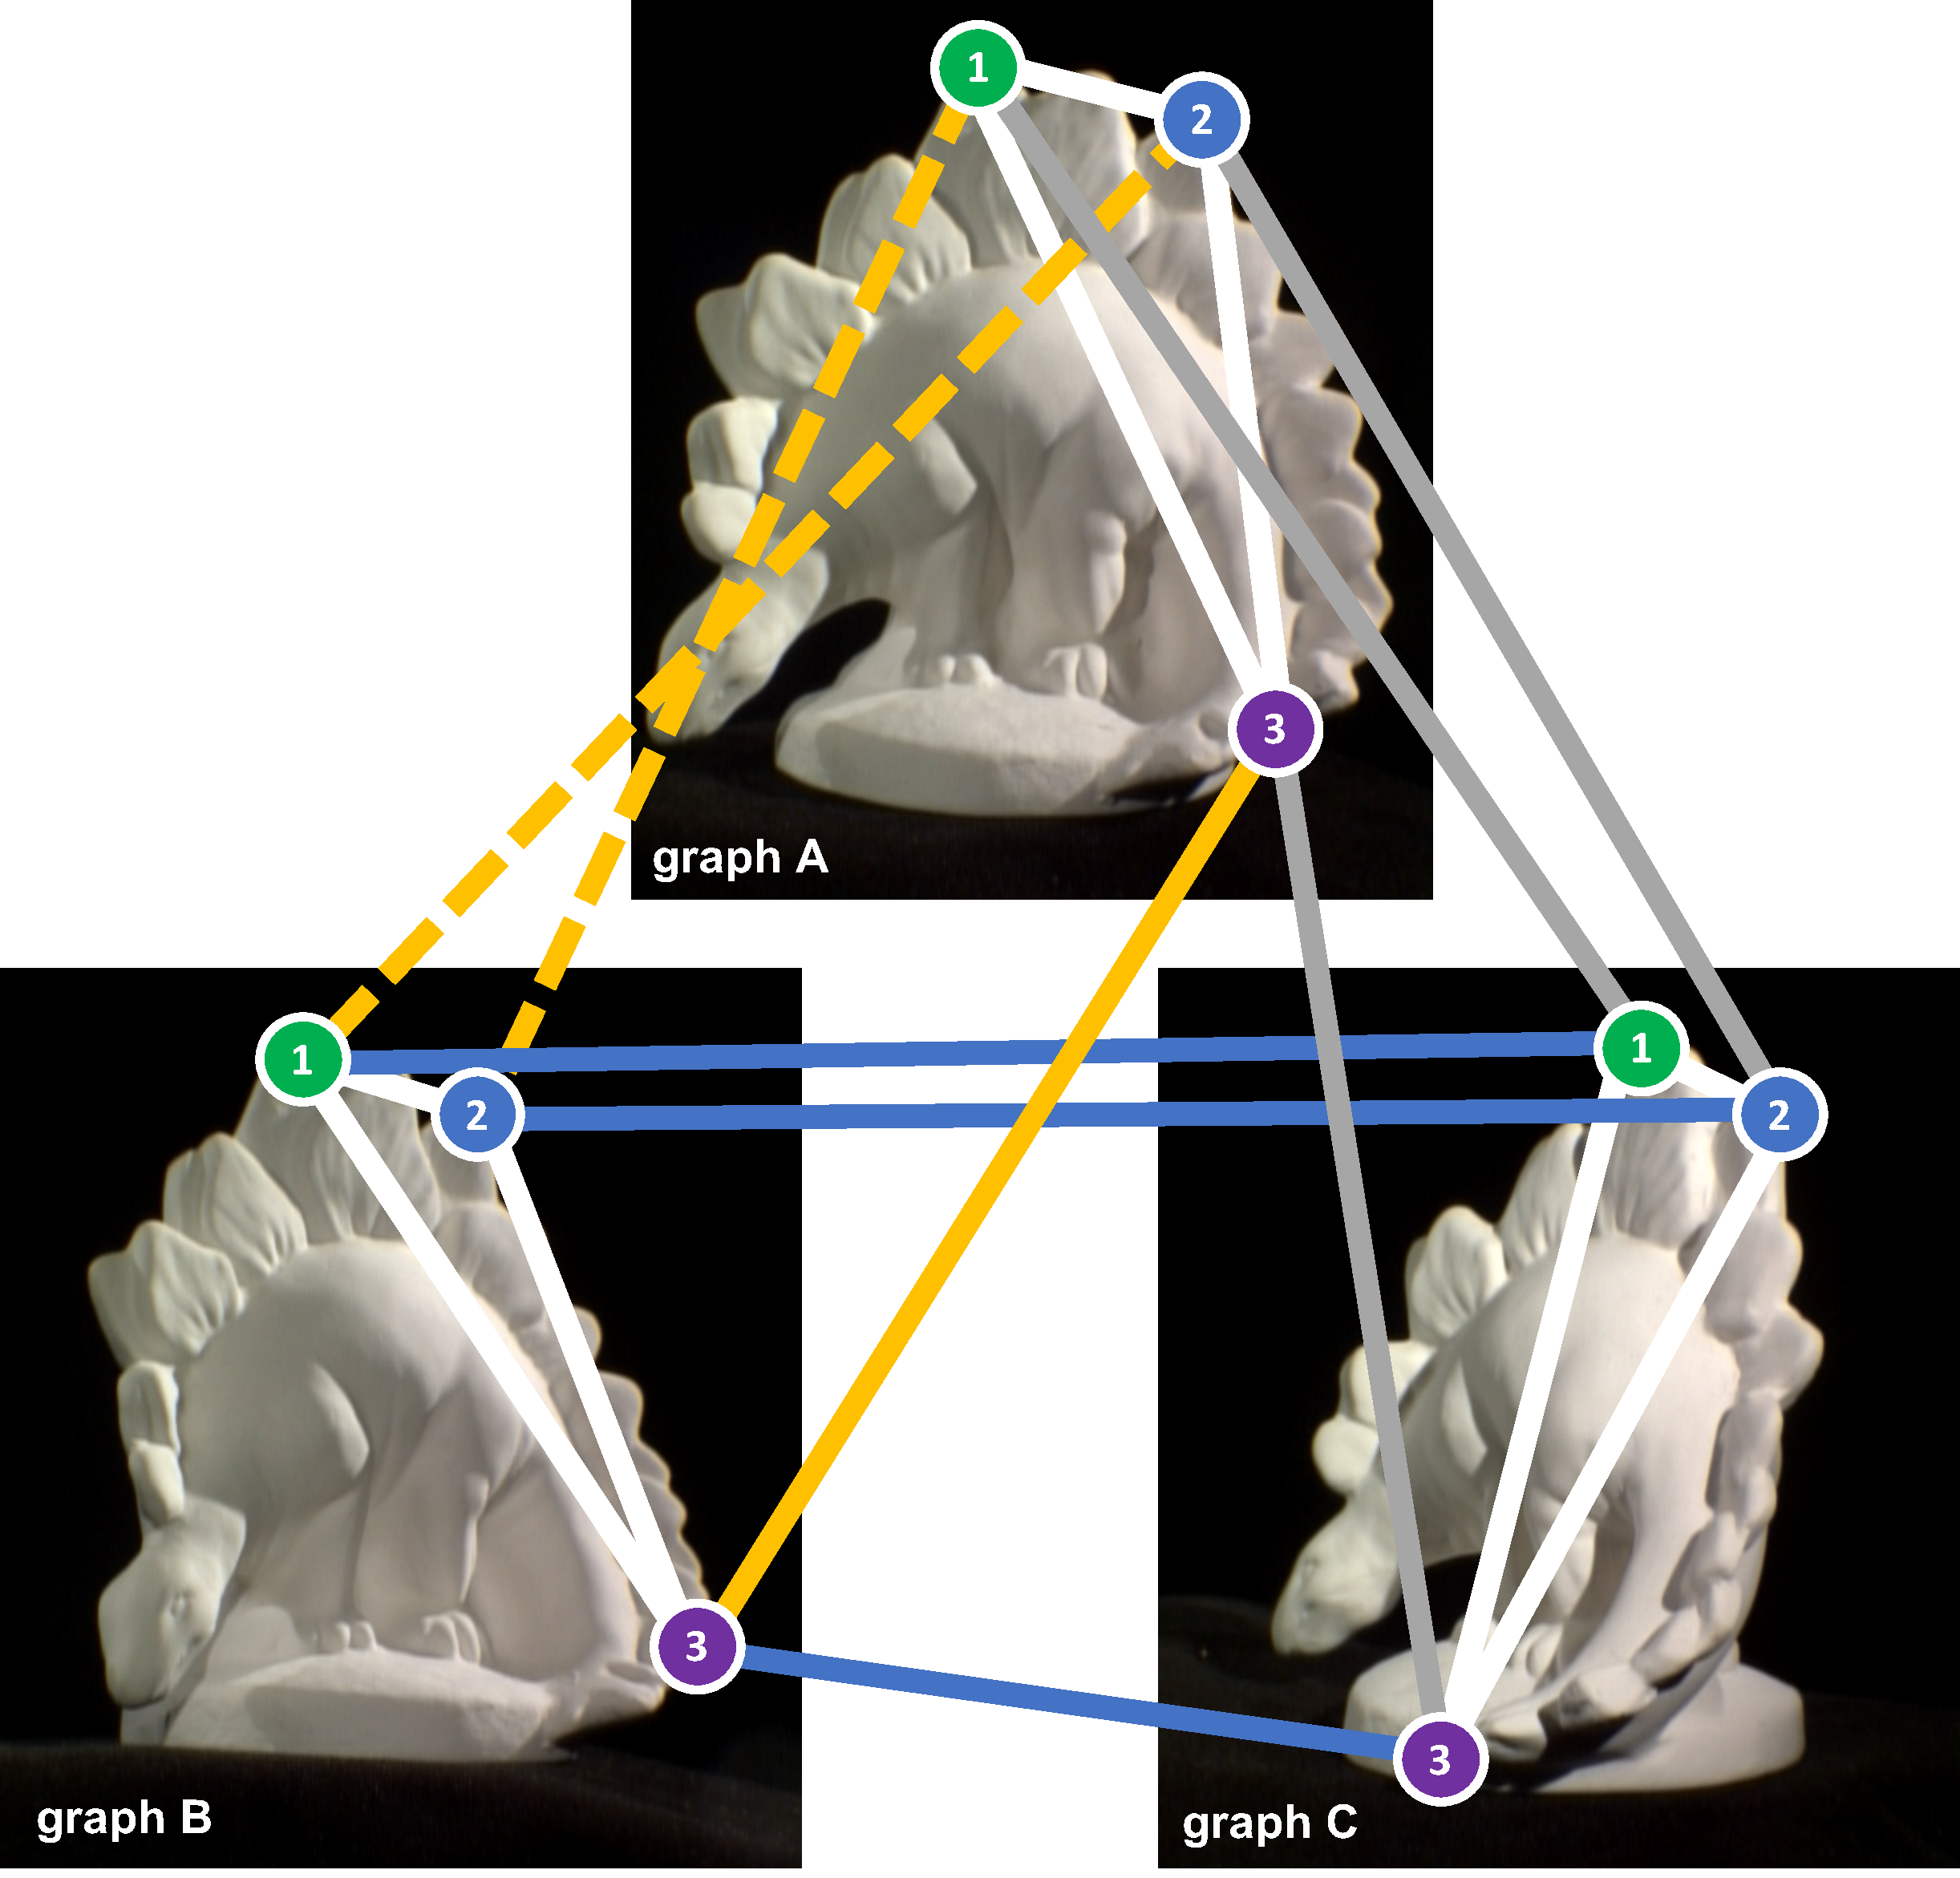
\includegraphics[width=0.7\columnwidth]{images/cycle-consistency.pdf}
    \caption{
        Illustration of cycle consistency in multi-graph matching (best viewed in color).
        Each graph $A$, $B$, $C$ comprises three nodes (green, blue, purple) and three edges (white lines).
        The true correspondence is indicated by the node colour and node labels 1, 2, 3.
        Matchings between pairs of graphs are shown by coloured lines ($A\leftrightarrow B)$ in yellow, $A \leftrightarrow C$ in gray, and $B \leftrightarrow C$ in blue).
        Wrong matchings are indicated by dashed lines.
        The multi-matching $A1 \leftrightarrow B2 \leftrightarrow C2 \leftrightarrow A2$ is not cycle consistent.
    }
    \label{fig:multi-graph-matching}
\end{figure}

\subsection{File Format}
The file format is derived from the one for graph matching described in Section~\ref{sec:graph-matching-file-format}.

\begin{fileformat}
gm (*$0$*) (*$1$*)
### graph matching problem for ###
### matching (*$0$*) with (*$1$*) ###
### as in Section(*$\text{~\ref{sec:graph-matching-file-format}}$*) ###

.
.
.

gm (*$K-2$*) (*$K-1$*)
### graph matching problem for ###
### matching (*$K-1$*) with (*$K-2$*) ###
### as in Section(*$\text{~\ref{sec:graph-matching-file-format}}$*) ###
\end{fileformat}

\subsection{Datasets}

\subsubsection[Hotel \& House]{Hotel \& House\footnote{\url{https://keeper.mpdl.mpg.de/f/d7ba7019eede485fb457/?dl=1}}}
In this experiment we consider the CMU house and hotel sequences.
$40\%$ of the points are outliers and the total number of points per image is $10$. 
For problem generation we have followed the protocol of [41], where further details are described.
Costs are computed as in~\cite{yan2015multi}.
In total there are 80 instances, 40 for house and 40 for hotel.

\subsubsection[Synthetic]{Synthetic\footnote{\url{https://keeper.mpdl.mpg.de/f/8ca51384836d40a09487/?dl=1}}}
Four different categories (complete, density, deform, outlier) of synthetic multi-graph matching problems with the number of point sets varying from 4 to 16 generated as in~\cite{yan2015multi}.
In total there are 160 instances, 40 from each category.

\subsubsection[Worms]{Worms\footnote{\url{https://keeper.mpdl.mpg.de/f/8b1385731fae4febb4fe/?dl=1}}}
Multi-graph matching instances generated from 30 images of C.\ elegans~\cite{kainmueller2014active}.
Points correspond to nuclei of the organism, which can number up to 558 per point set.
Instances have from 3 to 10 randomly selected point sets.
In total there are 400 instances, 50 per number of point sets.

\subsection{Algorithms}
\begin{description}[style=unboxed]
    \item[Permutation Synchronization~\cite{bernard2019synchronisation,pachauri2013solving}:]
        Non-negative matrix factorisation followed by Euclidean projection for binarization.
    \item[Alternating Graph matching~\cite{yan2013joint,zhou2015multi,yan2015consistency}:]
        Alternating optimization between graph matching solvers and a cycle consistency-enforcing component.
    \item[Graduated Consistency~\cite{yan2014graduated,yan2015multi}:]
        Iterative approximation of the graph matching objective with gradual consistency enforcement.
    \item[Matrix Decomposition~\cite{yan2015matrix}:]
         Matrix decomposition based formulation solved through convex optimization.
    \item[Factorized Matching~\cite{zhou2015factorized}:]
        Global alternating minimization approach via low-rank matrix recovery.
    \item[Semidefinite Optimization~\cite{kezurer2015tight}:]
        Semidefinite optimization problem formulation of multi-graph matching.
    \item[Fast Clustering~\cite{tron2017fast}:]
        Clustering-based formulation identifying multi-image matchings from a density function in feature space.
    \item[Tensor Power Iteration~\cite{shi2016tensor}:]
        Rank-1 tensor approximation solved via power iteration.
    \item[Mining Consistent Features~\cite{wang2018multi}:]
        Multi-graph matching by matching sparse feature sets and geometric consistency through low-rank constraints. 
    \item[DS*~\cite{bernard2018ds}:]
        A lifting-free convex relaxation approach.
    \item[Random Walk~\cite{park2019consistent}:]
        A multi-layer random walk synchronization approach.
    \item[Convex Message Passing~\cite{swoboda2019convex}:] Lagrange decomposition optimized with message passing. Cycle consistency is enforced via a cutting plane procedure that adds tightening subproblems.
    \item[HiPPi~\cite{bernard2019hippi}:]
        A higher-order projected power iteration method. 
\end{description}

